\def\regenfigs{0}
\documentclass[anonymous,sigconf,9pt]{acmart}

\usepackage{microtype}
\if\regenfigs1
\usepackage{tikz,pgfplots}
\usetikzlibrary{arrows.meta}
\usepgfplotslibrary{groupplots}
\usepgfplotslibrary{external}
\usepgfplotslibrary{colorbrewer}
\pgfplotsset{cycle list/Set1}
\usepgfplotslibrary{fillbetween}
\pgfplotsset{compat=1.18}
\pgfplotsset{
    tick align=outside,
    tick pos=left,
    xmajorgrids,
    x grid style={white},
    ymajorgrids,
    y grid style={white},
    axis line style={white},
    axis background/.style={fill=white!89.803921568627459!black},
    legend style={draw=none, fill=none},
    legend cell align=left,
}
\pgfkeys{/pgf/number format/.cd, 1000 sep={\,}}

\pgfplotsset{
    log x ticks with fixed point/.style={
        xticklabel={
            \pgfkeys{/pgf/fpu=true}
            \pgfmathparse{2^\tick}%
            \pgfmathprintnumber[fixed relative, precision=4]{\pgfmathresult}
            \pgfkeys{/pgf/fpu=false}
        }
    },
    log10 x ticks with fixed point/.style={
        xticklabel={
            \pgfkeys{/pgf/fpu=true}
            \pgfmathparse{10^\tick}%
            \pgfmathprintnumber[fixed relative, precision=3]{\pgfmathresult}
            \pgfkeys{/pgf/fpu=false}
        }
    },
    log y ticks with fixed point/.style={
        yticklabel={
            \pgfkeys{/pgf/fpu=true}
            \pgfmathparse{2^\tick}%
            \pgfmathprintnumber[fixed relative, precision=4]{\pgfmathresult}
            \pgfkeys{/pgf/fpu=false}
        }
    }
}
\fi

\begin{document}

\begin{figure}[tbp]
\if\regenfigs1
\begin{tikzpicture}
\begin{axis}[
    thick,
    xmode=log,
    %ymode=log,
    legend style={at={(0.9,0.4)},anchor=east},
    xlabel={\# atoms},
    ylabel={\% of peak performance},
    height=2in,
    width=\linewidth,
]
    \addplot+[mark=*] table[y expr={100*\thisrowno{1}/1335.066624}] {results/satlj_h100.txt};
    \addlegendentry{LJ};
    \addplot+[mark=square*] table[y expr={100*\thisrowno{1}/4.067584}] {results/satsnap_h100.txt};
    \addlegendentry{SNAP};
    \addplot+[mark=diamond*] table[y expr={100*\thisrowno{1}/11.378491}] {results/satreax_h100.txt};
    \addlegendentry{ReaxFF};
\end{axis}
\end{tikzpicture}
\else
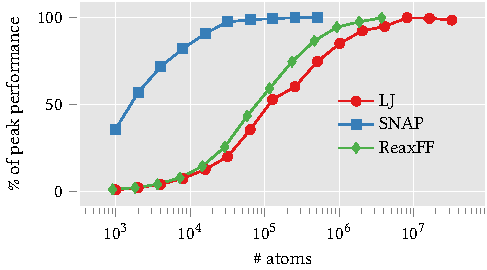
\includegraphics{generated-figures/paper-figure4.pdf}
\fi
\caption{Saturation of the normalized performance (atom-steps/s) on one NVIDIA H100 GPU for the three case studies. The much greater available parallelism of the ML-based SNAP potential allows it to run more efficiently for smaller system sizes. Note that ReaxFF ran out of HBM before reaching full saturation.}\label{fig:perfsat}
\end{figure}

\end{document}

